\documentclass[conference]{IEEEtran}
\IEEEoverridecommandlockouts

\usepackage{cite}
\usepackage{amsmath,amssymb,amsfonts}
\usepackage{graphicx}
\usepackage{textcomp}
\usepackage{xcolor}
\usepackage{listings}
\usepackage{url}
\usepackage{hyperref}
\usepackage{float}
\usepackage{booktabs}
\usepackage{tabularx}
\usepackage{tikz}
\usetikzlibrary{shapes.geometric, arrows.meta, positioning, fit, backgrounds}

% Code listing style
\lstdefinestyle{codestyle}{
    backgroundcolor=\color{gray!10},
    basicstyle=\ttfamily\scriptsize,
    breaklines=true,
    frame=single,
    numbers=left,
    numberstyle=\tiny\color{gray},
    keywordstyle=\color{blue},
    commentstyle=\color{green!50!black},
    stringstyle=\color{red!70!black},
    showstringspaces=false,
    tabsize=2
}
\lstset{style=codestyle}

\def\BibTeX{{\rm B\kern-.05em{\sc i\kern-.025em b}\kern-.08em
    T\kern-.1667em\lower.7ex\hbox{E}\kern-.125emX}}

\begin{document}

\title{PaperHub: A Serverless Cloud-Based Academic Conference Paper Submission System on AWS}

\author{\IEEEauthorblockN{Srinidhi Vutkoori}
\IEEEauthorblockA{Student ID: x25173243 \\
MSc in Cloud Computing \\
National College of Ireland, Dublin \\
x25173243@student.ncirl.ie}}

\maketitle

% ============================================================
% ABSTRACT
% ============================================================
\begin{abstract}
This paper presents the design, implementation, and deployment of PaperHub, a serverless cloud-based academic conference paper submission and peer review management system hosted on Amazon Web Services. The application enables conference organisers, authors, and reviewers to manage the complete lifecycle of academic paper submissions through a role-based web interface, encompassing conference creation, paper submission with PDF upload, structured peer review with scoring and recommendations, and automated status workflow management. The system leverages six AWS services programmatically, namely AWS Lambda for serverless compute, Amazon DynamoDB for NoSQL data storage, Amazon API Gateway for RESTful endpoint routing, Amazon S3 for PDF document storage and static website hosting, Amazon Simple Notification Service for status change email notifications, and AWS Identity and Access Management for fine-grained access control. A custom object-oriented Python library called confmanager-nci was developed and published, providing paper management, review coordination, conference administration, and paper formatting utilities with comprehensive validation logic. The application implements a role-based access control model distinguishing between author, reviewer, and administrator roles, with custom HMAC-based JWT authentication governing all API interactions. A CI/CD pipeline implemented through GitHub Actions automates testing, infrastructure provisioning, and deployment across all application tiers. The results demonstrate that serverless cloud architectures can effectively support complex multi-role academic workflow applications with robust state management and notification capabilities.
\end{abstract}

% ============================================================
% INTRODUCTION
% ============================================================
\section{Introduction}

The academic conference ecosystem relies heavily on paper submission and peer review processes that have traditionally been managed through email exchanges, shared spreadsheets, or expensive proprietary platforms such as EasyChair and OpenReview \cite{cloudpatterns}. These conventional approaches present significant challenges in terms of workflow consistency, reviewer coordination, status tracking, and transparency for all stakeholders involved in the conference management process. Cloud computing offers an opportunity to democratise access to robust conference management tools by leveraging scalable, pay-per-use infrastructure that eliminates the need for dedicated server management.

The motivation for this project arises from the observation that many small to medium-sized academic conferences and workshops lack access to affordable, feature-complete submission management systems. Existing solutions either impose per-paper fees that become prohibitive for student-run or departmental conferences, or require self-hosted infrastructure that demands ongoing maintenance and security management. By adopting the serverless computing paradigm available on AWS, this project demonstrates that a fully functional conference paper submission system with role-based access, peer review workflows, and automated notifications can be delivered at minimal operational cost \cite{serverless}.

The primary objectives of this project are threefold. First, to design and implement a serverless paper submission system supporting role-based access control for authors, reviewers, and administrators with custom HMAC-based JWT authentication. Second, to implement a complete paper lifecycle workflow including submission, peer review assignment, score aggregation, and status transition management with validation rules governing permitted state changes. Third, to develop a reusable Python library that encapsulates conference management domain logic including paper validation, review score processing, and conference scheduling utilities. The application employs six AWS services programmatically and demonstrates cloud-native architectural patterns including event-driven processing, role-based authorisation, and continuous deployment.

% ============================================================
% PROJECT SPECIFICATION AND REQUIREMENTS
% ============================================================
\section{Project Specification and Requirements}

\subsection{Functional Requirements}

The application satisfies the following functional requirements organised around the three primary user roles. First, the authentication and authorisation subsystem provides user registration and login with role assignment, where users are classified as authors, reviewers, or administrators. Authentication is managed through custom HMAC-based JWT tokens that encode the user's role, enabling the backend to enforce role-based access control on all API endpoints without maintaining server-side session state.

Second, the conference management subsystem allows administrators to create, update, and delete conferences with attributes including conference name, description, submission deadline, review deadline, and notification preferences. Administrators can view all conferences and manage the overall system configuration, while authors and reviewers can browse available conferences and their associated submission windows.

Third, the paper submission subsystem enables authors to submit papers to specific conferences by providing metadata including title, abstract, author list, and keywords, along with uploading the full paper as a PDF document to Amazon S3. Authors can view their submitted papers, update submissions before the review phase begins, and track the current status of each submission through their personalised dashboard.

Fourth, the peer review subsystem allows reviewers to access papers assigned to them, submit structured reviews comprising a numerical score on a scale of one to ten, written comments, and a recommendation category (accept, reject, or revision required). The system aggregates multiple review scores for each paper to inform the final acceptance decision by the administrator.

Fifth, the status workflow subsystem enforces a defined state machine for paper submissions, with permitted transitions from submitted to under\_review when reviewers are assigned, from under\_review to accepted, rejected, or revision\_required based on aggregated review outcomes, and from revision\_required back to submitted when authors resubmit. Amazon SNS notifications are triggered automatically on each status transition to inform the relevant authors of changes to their submissions.

\subsection{Non-Functional Requirements}

The non-functional requirements address scalability, security, availability, and cost efficiency. The serverless architecture provides automatic horizontal scaling through AWS Lambda, accommodating variable submission volumes that typically peak around conference deadlines \cite{awslambda}. Security is implemented through multiple layers: custom HMAC-based JWT authentication with role claims, IAM role-based access control for the Lambda execution environment restricting access to only the required AWS resources, CORS policies on API Gateway, and S3 bucket policies that enforce appropriate read and write permissions for PDF storage. Availability is ensured through the managed nature of all six AWS services within the eu-west-1 region, each providing built-in redundancy. Cost efficiency is achieved through Lambda's pay-per-invocation model and DynamoDB's on-demand billing, where charges accrue only during active submission and review periods.

% ============================================================
% ARCHITECTURE AND DESIGN
% ============================================================
\section{Architecture and Design}

PaperHub follows a serverless architecture pattern comprising three distinct tiers: a static frontend hosted on Amazon S3, a serverless API layer powered by AWS Lambda and Amazon API Gateway, and a data persistence layer using Amazon DynamoDB and Amazon S3 \cite{cloudpatterns}. This architecture was selected for its elimination of server management overhead, automatic scaling capabilities during peak submission periods, and cost-optimised pay-per-use billing that is particularly advantageous for conference systems with cyclical usage patterns.

\begin{figure}[H]
\centering
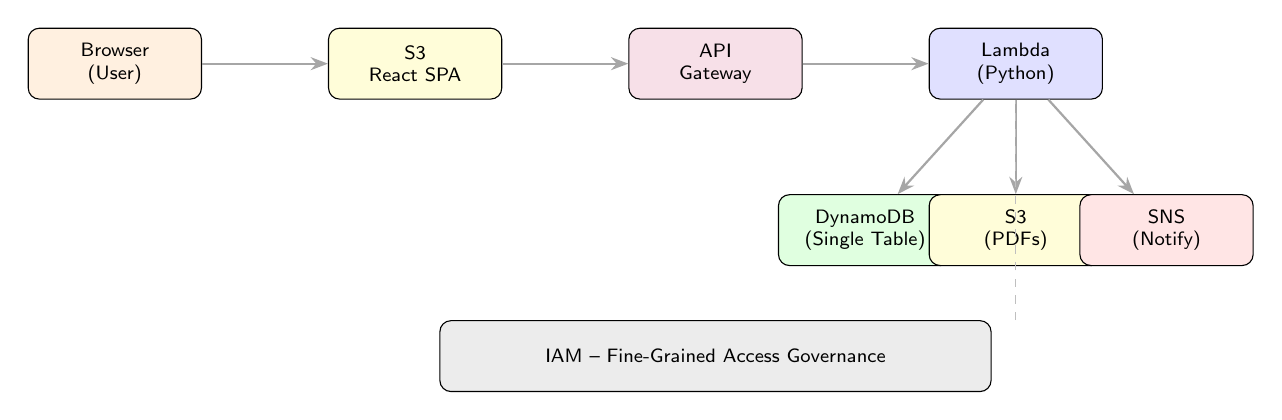
\begin{tikzpicture}[
    node distance=1.4cm and 1.6cm,
    box/.style={draw, rounded corners, minimum width=2.2cm, minimum height=0.9cm, align=center, font=\scriptsize\sffamily, fill=#1},
    box/.default={blue!8},
    arr/.style={-{Stealth[length=2.2mm]}, thick, color=gray!70},
    every node/.style={font=\scriptsize\sffamily}
]
    % Frontend tier
    \node[box=orange!12] (browser) {Browser\\(User)};
    \node[box=yellow!15, right=of browser] (s3fe) {S3\\React SPA};

    % API tier
    \node[box=purple!12, right=of s3fe] (apigw) {API\\Gateway};
    \node[box=blue!12, right=of apigw] (lambda) {Lambda\\(Python)};

    % Data tier - below lambda
    \node[box=green!12, below left=1.2cm and -0.3cm of lambda] (dynamo) {DynamoDB\\(Single Table)};
    \node[box=yellow!15, below=1.2cm of lambda] (s3pdf) {S3\\(PDFs)};
    \node[box=red!10, below right=1.2cm and -0.3cm of lambda] (sns) {SNS\\(Notify)};

    % IAM governance - spanning bottom
    \node[box=gray!15, below=2.8cm of apigw, minimum width=7cm] (iam) {IAM -- Fine-Grained Access Governance};

    % Arrows
    \draw[arr] (browser) -- (s3fe);
    \draw[arr] (s3fe) -- (apigw);
    \draw[arr] (apigw) -- (lambda);
    \draw[arr] (lambda) -- (dynamo);
    \draw[arr] (lambda) -- (s3pdf);
    \draw[arr] (lambda) -- (sns);

    % Dashed governance lines
    \draw[dashed, gray!50] (iam.north -| lambda) -- (lambda.south);
\end{tikzpicture}
\caption{PaperHub serverless architecture on AWS}
\label{fig:architecture}
\end{figure}

The frontend is a single-page React application built with Vite and styled using Tailwind CSS. The compiled static assets are deployed to an S3 bucket configured for static website hosting. The React application communicates with the backend exclusively through RESTful API calls routed through Amazon API Gateway, with JWT tokens attached to all authenticated requests via the Authorization header.

The API layer consists of a single AWS Lambda function that receives all incoming HTTP requests through API Gateway's proxy integration. The Lambda function implements a routing mechanism that dispatches requests to the appropriate handler based on the HTTP method, URL path, and the authenticated user's role extracted from the JWT token. This single-function approach simplifies deployment while the internal routing ensures clean separation of concerns between conference, paper, review, and authentication handlers. The Lambda function integrates with four additional AWS services: DynamoDB for data persistence, S3 for PDF storage, SNS for notifications, and IAM for execution permissions.

The data layer employs a single-table design in Amazon DynamoDB, using one table called \texttt{confpapers-prod} to store all entity types. Each item includes an \texttt{entityType} field that distinguishes between USER, CONFERENCE, PAPER, and REVIEW records, enabling polymorphic access patterns within a unified table. This single-table approach follows DynamoDB best practices by co-locating related entities to minimise the number of requests required for common operations \cite{awsdynamodb}. Items are keyed by their respective identifiers (userId, conferenceId, paperId, or reviewId), and a Global Secondary Index on the \texttt{entityType} field supports efficient retrieval of all items of a given type. DynamoDB was selected over relational alternatives because the primary access patterns involve retrieving individual entities by their identifier or querying items by entity type, both of which align efficiently with DynamoDB's key-value and secondary index query patterns. The PDF documents are stored in a dedicated S3 bucket with presigned URLs generated for secure, time-limited download access.

% ============================================================
% LIBRARY DESCRIPTION
% ============================================================
\section{Conference Manager Library}

The confmanager-nci library is a custom Python package developed specifically for this project to encapsulate the domain logic of conference paper submission and review management. The library follows object-oriented design principles with four primary classes, requiring no external dependencies beyond the Python standard library.

The library provides the following primary components. The \texttt{PaperManager} class handles paper lifecycle operations including submission validation, status transition enforcement, and metadata management. It validates that paper titles meet minimum length requirements, abstracts fall within acceptable word count ranges, and author lists contain at least one entry with valid affiliation information. The status transition logic ensures that only permitted state changes can occur, raising descriptive exceptions when invalid transitions are attempted.

The \texttt{ReviewManager} class coordinates the peer review process, providing review assignment tracking, score validation ensuring values fall within the one to ten range, recommendation validation against the permitted set (accept, reject, revision\_required), and score aggregation across multiple reviews for a single paper. The aggregation method computes weighted averages and determines consensus recommendations based on configurable thresholds.

The \texttt{ConferenceManager} class provides conference lifecycle utilities including deadline validation, submission window checking to determine whether a conference is currently accepting papers, and conference metadata formatting for display purposes. The \texttt{PaperFormatter} class supports multiple output formats for paper metadata including plain text summaries, structured JSON for API responses, and formatted citation strings.

The following code snippet demonstrates how the library's review aggregation is used within the application to determine paper acceptance decisions:

\begin{lstlisting}[language=Python, caption={ReviewManager usage for review score aggregation}]
from confmanager import ReviewManager

review_mgr = ReviewManager()

reviews = [
    {"reviewer_id": "r1", "score": 8,
     "recommendation": "accept",
     "comments": "Strong methodology"},
    {"reviewer_id": "r2", "score": 6,
     "recommendation": "revision_required",
     "comments": "Needs more experiments"},
    {"reviewer_id": "r3", "score": 7,
     "recommendation": "accept",
     "comments": "Well-written paper"},
]
# Aggregate review scores and recommendations
result = review_mgr.aggregate_reviews(reviews)
# Returns: {avg_score: 7.0, recommendation: "accept",
#           review_count: 3, consensus: True}
status = review_mgr.determine_status(result)
# Returns: "accepted"
\end{lstlisting}

The library includes 80 unit tests implemented with pytest, covering all four classes comprehensively. The test suite validates paper submission edge cases including empty fields and excessively long abstracts, review score boundary conditions, status transition validity for all possible state combinations, conference deadline enforcement, and formatter output correctness across all supported formats. The library is installed as a dependency in the Lambda deployment package and its test suite is executed as a mandatory gate in the CI/CD pipeline.

% ============================================================
% CLOUD SERVICES
% ============================================================
\section{Cloud-Based Services}

The application integrates six AWS services, each serving a distinct purpose within the serverless architecture. This section provides a critical analysis and justification for each service selection.

\subsection{AWS Lambda}

AWS Lambda provides the serverless compute environment for the backend API, executing the Python 3.11 handler function in response to API Gateway events \cite{awslambda}. Lambda was selected over container-based alternatives such as AWS Fargate or Elastic Beanstalk because the event-driven request pattern of a conference submission system, which experiences variable load with peaks around submission deadlines, aligns naturally with Lambda's automatic scaling and pay-per-request pricing. The function is configured with 512 MB of memory and a 30-second timeout, providing sufficient resources for PDF processing, JWT validation, and database operations. A potential limitation is Lambda's cold start latency, which can introduce delays of several hundred milliseconds for the first request after a period of inactivity; however, this is acceptable for a conference management system where sub-second response times are not critical.

\subsection{Amazon DynamoDB}

Amazon DynamoDB provides a fully managed NoSQL database for storing all application data in a single table called \texttt{confpapers-prod} \cite{awsdynamodb}. The table uses a single-table design pattern where each item includes an \texttt{entityType} attribute (USER, CONFERENCE, PAPER, or REVIEW) to distinguish between record types, enabling polymorphic data access within a unified table structure. This approach follows DynamoDB best practices by reducing the number of tables to manage and allowing related data to be co-located for efficient access. The table uses on-demand billing mode, which is ideal for conference systems where write volume spikes during submission windows and drops to near zero between conferences. DynamoDB was preferred over Amazon RDS because the application's access patterns are predominantly key-value lookups and single-table queries that do not require complex relational joins. A Global Secondary Index on the \texttt{entityType} attribute enables efficient retrieval of all items of a given type, such as listing all conferences or all papers.

\subsection{Amazon API Gateway}

Amazon API Gateway provides the HTTP endpoint layer that routes incoming requests to the Lambda function using proxy integration \cite{awsapigateway}. The REST API is configured with a catch-all \texttt{\{proxy+\}} resource that forwards all HTTP methods and paths to the single Lambda handler. API Gateway was selected for its native Lambda integration, built-in request throttling that protects against abuse during high-volume submission periods, and ability to handle CORS preflight OPTIONS requests at the gateway level. An alternative approach using Application Load Balancer was considered but rejected due to its hourly billing model, which would incur costs even during inactive periods between conferences.

\subsection{Amazon S3}

Amazon S3 serves a dual purpose in the architecture: storing uploaded PDF paper documents in a dedicated bucket and hosting the compiled React frontend as a static website in a separate bucket \cite{awss3}. The PDF storage bucket is configured with private access by default, with the Lambda function generating presigned URLs that grant time-limited download access to authorised users. This approach ensures that paper documents are not publicly accessible while still allowing reviewers and administrators to download them through the application interface. The frontend bucket is configured with public access and static website hosting enabled.

\subsection{Amazon SNS}

Amazon Simple Notification Service provides the publish-subscribe messaging infrastructure for paper status change notifications \cite{awssns}. An SNS topic serves as the central notification channel, and authors receive email notifications when the status of their submitted papers changes. When a paper transitions from under\_review to accepted, rejected, or revision\_required, the Lambda function publishes a notification message containing the paper title, new status, and any reviewer comments to the SNS topic. SNS was chosen over Amazon SES because SNS natively supports topic-based fan-out and subscription management, which aligns well with the requirement to notify multiple stakeholders about conference-wide announcements in addition to individual paper status updates.

\begin{lstlisting}[language=Python, caption={SNS notification on paper status change}]
def notify_status_change(paper, new_status):
    message = (
        f"Paper Status Update - PaperHub\n\n"
        f"Paper: {paper['title']}\n"
        f"Conference: {paper['conference_name']}\n"
        f"New Status: {new_status}\n"
        f"Updated: {datetime.utcnow().isoformat()}\n"
    )
    sns.publish(
        TopicArn=SNS_TOPIC_ARN,
        Subject=f"Paper Status: {new_status.upper()}",
        Message=message
    )
\end{lstlisting}

\subsection{AWS IAM}

AWS Identity and Access Management provides the security foundation for the serverless architecture by defining the Lambda function's execution role and its associated permission policies \cite{awsiam}. The IAM role grants the Lambda function precisely scoped permissions to read and write to the DynamoDB table, put and get objects in the S3 PDF bucket, publish messages to the SNS topic, and write logs to CloudWatch Logs. The principle of least privilege is followed by restricting each permission to the specific resource ARN rather than granting broad wildcard access. IAM was essential rather than optional because without properly configured execution roles, the Lambda function would be unable to interact with any other AWS service, making it the foundational security service upon which all other integrations depend.

% ============================================================
% IMPLEMENTATION
% ============================================================
\section{Implementation}

The implementation follows a clean separation between the frontend React application, the serverless Lambda backend with custom HMAC-based JWT authentication, and the custom Python library. This section documents the implementation of each major component.

\subsection{Backend API and CRUD Operations}

The Lambda function implements role-aware API routes through a path-based routing mechanism. All authenticated endpoints extract the JWT token from the Authorization header, verify the HMAC signature, and enforce role-based access before processing the request. Table~\ref{tab:endpoints} summarises the primary API endpoints.

\begin{table}[H]
\centering
\caption{PaperHub REST API Endpoints}
\label{tab:endpoints}
\begin{tabular}{|l|l|l|}
\hline
\textbf{Method} & \textbf{Endpoint} & \textbf{Description} \\
\hline
POST & /auth/register & Register new user \\
POST & /auth/login & Login, return JWT \\
\hline
GET & /conferences & List conferences \\
POST & /conferences & Create conference (admin) \\
PUT & /conferences/\{id\} & Update conference (admin) \\
DELETE & /conferences/\{id\} & Delete conference (admin) \\
\hline
POST & /papers & Submit paper (author) \\
GET & /papers & List user's papers \\
GET & /papers/\{id\} & Get paper details \\
PUT & /papers/\{id\}/status & Update status (admin) \\
\hline
POST & /reviews & Submit review (reviewer) \\
GET & /reviews/\{paperId\} & Get paper reviews \\
\hline
GET & /dashboard & Role-based dashboard \\
\hline
\end{tabular}
\end{table}

A critical implementation detail involved the custom HMAC-based JWT authentication, which was implemented without relying on the PyJWT library. The system constructs tokens manually by base64-encoding the header and payload segments, then signing them with HMAC-SHA256. Token verification recomputes the signature and uses a constant-time comparison to prevent timing attacks. The status transition validation leverages the confmanager-nci library to ensure that only valid workflow transitions are permitted:

\begin{lstlisting}[language=Python, caption={Custom HMAC-based JWT and status transition}]
import hmac, hashlib, base64, json, time

JWT_SECRET = os.environ.get("JWT_SECRET",
    "confpapers-secret-2026")

def _b64_encode(data):
    return base64.urlsafe_b64encode(
        json.dumps(data).encode()
    ).decode().rstrip("=")

def generate_token(user_id, username, email, role):
    header = {"alg": "HS256", "typ": "JWT"}
    payload = {
        "userId": user_id, "username": username,
        "email": email, "role": role,
        "exp": int(time.time()) + 86400,
        "iat": int(time.time()),
    }
    segments = _b64_encode(header) + "." \
        + _b64_encode(payload)
    sig = hmac.new(JWT_SECRET.encode(),
        segments.encode(), hashlib.sha256).digest()
    return segments + "." + base64.urlsafe_b64encode(
        sig).decode().rstrip("=")

def decode_token(token):
    parts = token.split(".")
    if len(parts) != 3:
        return None
    segments = parts[0] + "." + parts[1]
    expected = hmac.new(JWT_SECRET.encode(),
        segments.encode(), hashlib.sha256).digest()
    expected_b64 = base64.urlsafe_b64encode(
        expected).decode().rstrip("=")
    if not hmac.compare_digest(expected_b64, parts[2]):
        return None
    return _b64_decode(parts[1])
\end{lstlisting}

\subsection{Frontend Implementation}

The frontend is implemented as a single-page React application with Vite as the build tool and Tailwind CSS for styling. The application features role-aware navigation that dynamically adjusts the available menu items and dashboard views based on the authenticated user's role. Authors see their submission history with status indicators, reviewers see assigned papers awaiting review with score entry forms, and administrators see an overview of all conferences, papers, and aggregate review statistics.

The paper submission form includes a drag-and-drop PDF upload component that converts the file to base64 for transmission to the Lambda backend, which then stores the document in the S3 PDF bucket. The review submission interface presents a structured form with a numeric score slider (one to ten), a recommendation dropdown, and a free-text comments area with minimum length validation.

\subsection{Testing}

The confmanager-nci library includes 80 automated unit tests implemented with pytest, distributed across five test modules covering the four primary classes. The tests validate paper submission with boundary conditions on title length and abstract word count, review score validation at boundary values of one and ten, all permitted and prohibited status transitions in the paper workflow state machine, conference deadline enforcement including edge cases at exact deadline times, reviewer assignment with conflict-of-interest avoidance, acceptance rate calculations, and formatter output consistency across all supported formats including CSV export, acceptance letters, and rejection letters. The CI/CD pipeline executes this test suite as a mandatory gate before deployment proceeds.

% ============================================================
% CI/CD AND DEPLOYMENT
% ============================================================
\section{Continuous Integration, Delivery and Deployment}

The application source code is maintained in a GitHub repository at \url{https://github.com/srinidhivutkoori/cpp}. A comprehensive CI/CD pipeline was implemented using GitHub Actions, triggered automatically on every push to the main branch. The pipeline consists of three sequential jobs that collectively automate testing, infrastructure provisioning, and application deployment.

The first job, \texttt{test-library}, installs the confmanager-nci library in editable mode and executes the full pytest suite of 80 unit tests. Only when all tests pass does the pipeline proceed to backend deployment.

The second job, \texttt{deploy-backend}, provisions all required AWS infrastructure using the AWS CLI. This includes creating the DynamoDB table (\texttt{confpapers-prod}) with on-demand billing and appropriate key schema supporting the single-table design, creating S3 buckets with CORS configurations for PDF storage and frontend hosting, creating an IAM role with policies scoped to the specific DynamoDB table, S3 buckets, SNS topic, and CloudWatch log groups, creating an SNS topic for status change notifications, packaging the Lambda function code with all dependencies including the confmanager-nci library, and configuring API Gateway with proxy integration. All resource creation commands are idempotent, using existence checks to handle repeated deployments safely.

The third job, \texttt{deploy-frontend}, retrieves the API Gateway URL from the deployed backend, builds the React application with the API URL injected as an environment variable, and synchronises the compiled assets to the frontend S3 bucket with appropriate cache control headers.

The pipeline requires AWS\_ACCESS\_KEY\_ID and AWS\_SECRET\_ACCESS\_KEY as GitHub repository secrets. All other configuration values including resource ARNs and API URLs are derived dynamically during pipeline execution, ensuring the deployment is fully reproducible from a clean AWS account.

The deployed application is accessible at the following URLs:

\begin{itemize}
    \item \textbf{Frontend:} \url{http://confpapers-frontend-prod-srinidhi.s3-website-eu-west-1.amazonaws.com}
    \item \textbf{PyPI Package:} \url{https://pypi.org/project/confmanager-nci/1.0.0/}
    \item \textbf{GitHub Repository:} \url{https://github.com/srinidhivutkoori/cpp}
\end{itemize}

Demo credentials are pre-seeded for evaluation purposes:

\begin{itemize}
    \item \textbf{Admin:} admin@paperhub.demo / Admin1234!
    \item \textbf{Reviewer:} reviewer@paperhub.demo / Review1234!
    \item \textbf{Author:} author@paperhub.demo / Author1234!
\end{itemize}

% ============================================================
% CONCLUSIONS
% ============================================================
\section{Conclusions}

This project successfully demonstrates the development and deployment of a serverless cloud-native application that integrates six AWS services to deliver a comprehensive academic conference paper submission and peer review management platform. PaperHub provides role-based access for authors, reviewers, and administrators, structured peer review with score aggregation, enforced status workflow transitions, and automated email notifications, all without requiring any server infrastructure management.

Several key findings emerged during the development process. First, implementing role-based access control through custom HMAC-based JWT tokens proved effective for a serverless architecture where traditional session-based authentication is impractical. By constructing tokens manually with HMAC-SHA256 signatures and encoding the user's role directly in the payload, the Lambda function can make authorisation decisions without additional database lookups or third-party dependencies on every request. The use of constant-time comparison via \texttt{hmac.compare\_digest} also provides protection against timing-based attacks on token verification.

Second, the status transition validation implemented through the confmanager-nci library proved essential for maintaining data integrity in the paper workflow. Without programmatic enforcement of the state machine, it would be possible for papers to reach invalid states through concurrent API calls or client-side manipulation. The library's transition validation serves as a critical guard that operates independently of the frontend, ensuring consistency regardless of how the API is invoked.

Third, the single-table DynamoDB design using an \texttt{entityType} discriminator field proved effective for modelling the polymorphic data requirements of the conference management domain. By co-locating USER, CONFERENCE, PAPER, and REVIEW entities within a single table, the application minimises the number of DynamoDB tables to provision and manage, while the Global Secondary Index on \texttt{entityType} supports efficient retrieval of homogeneous collections when needed.

The main limitations of the current implementation include the absence of reviewer assignment automation, which currently requires manual allocation by administrators. A future enhancement could integrate an algorithm that matches reviewers to papers based on keyword similarity between reviewer expertise profiles and paper abstracts. Additionally, the current PDF storage does not include plagiarism detection or format validation, which would be valuable additions for a production conference management system. The serverless architecture provides a solid foundation for these extensions, as additional Lambda functions and services such as Amazon Textract for document analysis could be integrated incrementally.

% ============================================================
% REFERENCES
% ============================================================
\begin{thebibliography}{00}

\bibitem{cloudpatterns} C. Richardson, ``Microservices Patterns: With Examples in Java,'' Manning Publications, 2018.

\bibitem{serverless} P. Sbarski, ``Serverless Architectures on AWS: With Examples Using AWS Lambda,'' 2nd ed., Manning Publications, 2022.

\bibitem{awslambda} Amazon Web Services, ``AWS Lambda Developer Guide,'' 2024. [Online]. Available: https://docs.aws.amazon.com/lambda/

\bibitem{awsdynamodb} Amazon Web Services, ``Amazon DynamoDB Developer Guide,'' 2024. [Online]. Available: https://docs.aws.amazon.com/dynamodb/

\bibitem{awsapigateway} Amazon Web Services, ``Amazon API Gateway Developer Guide,'' 2024. [Online]. Available: https://docs.aws.amazon.com/apigateway/

\bibitem{awss3} Amazon Web Services, ``Amazon Simple Storage Service (S3) Documentation,'' 2024. [Online]. Available: https://docs.aws.amazon.com/s3/

\bibitem{awssns} Amazon Web Services, ``Amazon Simple Notification Service Developer Guide,'' 2024. [Online]. Available: https://docs.aws.amazon.com/sns/

\bibitem{awsiam} Amazon Web Services, ``AWS Identity and Access Management User Guide,'' 2024. [Online]. Available: https://docs.aws.amazon.com/iam/

\bibitem{react} Meta Platforms, ``React Documentation,'' 2024. [Online]. Available: https://react.dev/

\bibitem{vite} E. You, ``Vite: Next Generation Frontend Tooling,'' 2024. [Online]. Available: https://vitejs.dev/

\end{thebibliography}

\end{document}
